\tikzset{
  place/.style={
    circle,
    thick,
    draw=black!100, % draw=blue!75,
    % fill=blue!20,
    minimum size=0.3mm
  },
  transition/.style={
    rectangle,
    thick,
    fill=black,
    minimum width=2mm,
    inner ysep=0.7pt,
  },
  timedtransition/.style={
    rectangle,
    thick,
    fill=black,
    minimum width=4mm,
    inner ysep=0.5pt
  },
  inhibitor/.style={-o},
  text=\small
}  
\chapter{Complete Petri Net} 
\label{chap:CompletePetriNet}

\begin{longtable}{M{5cm}M{10cm}}
\caption{Complete Places.}
\\
Places & Meaning\\
\hline
\endfirsthead
\multicolumn{2}{l}{Continued from previous page} \\
\hline

Places & Meaning \\

\hline
\endhead
\hline\multicolumn{2}{r}{Continued on next page} \\
\endfoot
\endlastfoot
\hline
\hyperlink{completeNet:p0m1}{\hypertarget{completeTable:p0m1}{$p_{0}$}} & System Stopped\\
\hyperlink{completeNet:p1}{\hypertarget{completeTable:p1}{$p_{1}$}}, \hyperlink{completeNet:p31}{\hypertarget{completeTable:p31}{$p_{31}$}} & Retract MAG1's Cylinder *\\
\hyperlink{completeNet:p2}{\hypertarget{completeTable:p2}{$p_{2}$}}, \hyperlink{completeNet:p32}{\hypertarget{completeTable:p32}{$p_{32}$}} & MAG1's Cylinder Retracted\\
\hyperlink{completeNet:p3}{\hypertarget{completeTable:p3}{$p_{3}$}}, \hyperlink{completeNet:p54}{\hypertarget{completeTable:p54}{$p_{54}$}} & Retract MAG2's Cylinder *\\
\hyperlink{completeNet:p4}{\hypertarget{completeTable:p4}{$p_{4}$}}, \hyperlink{completeNet:p55}{\hypertarget{completeTable:p55}{$p_{55}$}} & MAG2's Cylinder Retracted\\
\hyperlink{completeNet:p5}{\hypertarget{completeTable:p5}{$p_{5}$}}, \hyperlink{completeNet:p38}{\hypertarget{completeTable:p38}{$p_{38}$}}, \hyperlink{completeNet:p64}{\hypertarget{completeTable:p64}{$p_{64}$}} & Retract Right Discharge Cylinder *\\
\hyperlink{completeNet:p6}{\hypertarget{completeTable:p6}{$p_{6}$}} & Right Discharge Cylinder Retracted\\
\hyperlink{completeNet:p7}{\hypertarget{completeTable:p7}{$p_{7}$}} & Retract Center Discharge Cylinder\\
\hyperlink{completeNet:p8}{\hypertarget{completeTable:p8}{$p_{8}$}} & Center Discharge Cylinder Retracted\\
\hyperlink{completeNet:p9}{\hypertarget{completeTable:p9}{$p_{9}$}}, \hyperlink{completeNet:p46}{\hypertarget{completeTable:p46}{$p_{46}$}}, \hyperlink{completeNet:p60}{\hypertarget{completeTable:p60}{$p_{60}$}} & Retract Left Discharge Cylinder *\\
\hyperlink{completeNet:p10}{\hypertarget{completeTable:p10}{$p_{10}$}} & Left Discharge Cylinder Retracted\\
\hyperlink{completeNet:p11}{\hypertarget{completeTable:p11}{$p_{11}$}} & Turn Conveyor Belt On (Reverse)\\
\hyperlink{completeNet:p12}{\hypertarget{completeTable:p12}{$p_{12}$}} & No Pieces On Conveyor Belt\\
\hyperlink{completeNet:p13}{\hypertarget{completeTable:p13}{$p_{13}$}} & Reset Variables\\
\hyperlink{completeNet:p14}{\hypertarget{completeTable:p14}{$p_{14}$}} & Raise Press\\
\hyperlink{completeNet:p15}{\hypertarget{completeTable:p15}{$p_{15}$}} & Open Safety Door\\
\hyperlink{completeNet:p16}{\hypertarget{completeTable:p16}{$p_{16}$}} & Extend Assembly Unit Holder\\
\hyperlink{completeNet:p17}{\hypertarget{completeTable:p17}{$p_{17}$}} & Assembly Unit Ready\\
\hyperlink{completeNet:p18}{\hypertarget{completeTable:p18}{$p_{18}$}} & Arm Lowered and Retracted, and Storage Unit Retracted\\
\hyperlink{completeNet:p19}{\hypertarget{completeTable:p19}{$p_{19}$}}, \hyperlink{completeNet:p109}{\hypertarget{completeTable:p109}{$p_{109}$}}, \hyperlink{completeNet:p134}{\hypertarget{completeTable:p134}{$p_{134}$}} & Move Storage Unit to the Right\\
\hyperlink{completeNet:p20}{\hypertarget{completeTable:p20}{$p_{20}$}} & Storage Unit ready ( horizontal )\\
\hyperlink{completeNet:p21}{\hypertarget{completeTable:p21}{$p_{21}$}} & Move Storage Device Downwards\\
\hyperlink{completeNet:p22}{\hypertarget{completeTable:p22}{$p_{22}$}} & Storage Unit ready ( vertical )\\
\hyperlink{completeNet:p23}{\hypertarget{completeTable:p23}{$p_{23}$}} & Rotate Arm CCW\\
\hyperlink{completeNet:p24}{\hypertarget{completeTable:p24}{$p_{24}$}}, \hyperlink{completeNet:p105}{\hypertarget{completeTable:p105}{$p_{105}$}} & Turn HSC Off ( Arm Stopped )\\
\hyperlink{completeNet:p25}{\hypertarget{completeTable:p25}{$p_{25}$}} & Rotate Arm CW\\
\hyperlink{completeNet:p26}{\hypertarget{completeTable:p26}{$p_{26}$}}, \hyperlink{completeNet:p107}{\hypertarget{completeTable:p107}{$p_{107}$}} & Arm Stopped facing conveyor belt\\
\hyperlink{completeNet:p27}{\hypertarget{completeTable:p27}{$p_{27}$}} & System Ready\\
\hyperlink{completeNet:p29}{\hypertarget{completeTable:p29}{$p_{29}$}} & MAG1 Not Empty\\
\hyperlink{completeNet:p30}{\hypertarget{completeTable:p30}{$p_{30}$}} & Extend MAG1's Cylinder *\\
\hyperlink{completeNet:p33}{\hypertarget{completeTable:p33}{$p_{33}$}}, \hyperlink{completeNet:p36}{\hypertarget{completeTable:p36}{$p_{36}$}}, \hyperlink{completeNet:p39}{\hypertarget{completeTable:p39}{$p_{39}$}}, \hyperlink{completeNet:p44}{\hypertarget{completeTable:p44}{$p_{44}$}}, \hyperlink{completeNet:p47}{\hypertarget{completeTable:p47}{$p_{47}$}}, \hyperlink{completeNet:p48}{\hypertarget{completeTable:p48}{$p_{48}$}}, \hyperlink{completeNet:p56}{\hypertarget{completeTable:p56}{$p_{56}$}}, \hyperlink{completeNet:p58}{\hypertarget{completeTable:p58}{$p_{58}$}}, \hyperlink{completeNet:p62}{\hypertarget{completeTable:p62}{$p_{62}$}}, \hyperlink{completeNet:p66}{\hypertarget{completeTable:p66}{$p_{66}$}}, \hyperlink{completeNet:p70}{\hypertarget{completeTable:p70}{$p_{70}$}}, \hyperlink{completeNet:p71}{\hypertarget{completeTable:p71}{$p_{71}$}} & Turn Conveyor Belt On\\
\hyperlink{completeNet:p34}{\hypertarget{completeTable:p34}{$p_{34}$}}, \hyperlink{completeNet:p42}{\hypertarget{completeTable:p42}{$p_{42}$}}, \hyperlink{completeNet:p57}{\hypertarget{completeTable:p57}{$p_{57}$}}, \hyperlink{completeNet:p69}{\hypertarget{completeTable:p69}{$p_{69}$}}, \hyperlink{completeNet:p110}{\hypertarget{completeTable:p110}{$p_{110}$}}, \hyperlink{completeNet:p117}{\hypertarget{completeTable:p117}{$p_{117}$}}, \hyperlink{completeNet:p129}{\hypertarget{completeTable:p129}{$p_{129}$}}, \hyperlink{completeNet:p138}{\hypertarget{completeTable:p138}{$p_{138}$}}, \hyperlink{completeNet:p146}{\hypertarget{completeTable:p146}{$p_{146}$}} & \\
\hyperlink{completeNet:p35}{\hypertarget{completeTable:p35}{$p_{35}$}} & Plastic Half-cube\\
\hyperlink{completeNet:p37}{\hypertarget{completeTable:p37}{$p_{37}$}}, \hyperlink{completeNet:p63}{\hypertarget{completeTable:p63}{$p_{63}$}} & Extend Right Discharge Cylinder *\\
\hyperlink{completeNet:p40}{\hypertarget{completeTable:p40}{$p_{40}$}}, \hyperlink{completeNet:p67}{\hypertarget{completeTable:p67}{$p_{67}$}} & Extend Center Discharge Cylinder *\\
\hyperlink{completeNet:p41}{\hypertarget{completeTable:p41}{$p_{41}$}}, \hyperlink{completeNet:p68}{\hypertarget{completeTable:p68}{$p_{68}$}} & Retract Center Discharge Cylinder *\\
\hyperlink{completeNet:p43}{\hypertarget{completeTable:p43}{$p_{43}$}}, \hyperlink{completeNet:p61}{\hypertarget{completeTable:p61}{$p_{61}$}} & Metal Half-cube\\
\hyperlink{completeNet:p45}{\hypertarget{completeTable:p45}{$p_{45}$}}, \hyperlink{completeNet:p59}{\hypertarget{completeTable:p59}{$p_{59}$}} & Extend Left Discharge Cylinder *\\
\hyperlink{completeNet:p49}{\hypertarget{completeTable:p49}{$p_{49}$}} & Metal Half-cube Ready\\
\hyperlink{completeNet:p50}{\hypertarget{completeTable:p50}{$p_{50}$}}, \hyperlink{completeNet:p73}{\hypertarget{completeTable:p73}{$p_{73}$}} & Conveyor Belt Stopped\\
\hyperlink{completeNet:p52}{\hypertarget{completeTable:p52}{$p_{52}$}} & MAG2 Not Empty\\
\hyperlink{completeNet:p53}{\hypertarget{completeTable:p53}{$p_{53}$}} & Extend MAG2's Cylinder *\\
\hyperlink{completeNet:p65}{\hypertarget{completeTable:p65}{$p_{65}$}} & White Half-Cube\\
\hyperlink{completeNet:p72}{\hypertarget{completeTable:p72}{$p_{72}$}} & Plastic Half-cube Ready\\
\hyperlink{completeNet:p75}{\hypertarget{completeTable:p75}{$p_{75}$}} & Raise and Extend Arm, and Turn Vacuum On\\
\hyperlink{completeNet:p76}{\hypertarget{completeTable:p76}{$p_{76}$}}, \hyperlink{completeNet:p81}{\hypertarget{completeTable:p81}{$p_{81}$}}, \hyperlink{completeNet:p94}{\hypertarget{completeTable:p94}{$p_{94}$}}, \hyperlink{completeNet:p101}{\hypertarget{completeTable:p101}{$p_{101}$}} & Extend Arm and Turn Vacuum On\\
\hyperlink{completeNet:p77}{\hypertarget{completeTable:p77}{$p_{77}$}}, \hyperlink{completeNet:p80}{\hypertarget{completeTable:p80}{$p_{80}$}}, \hyperlink{completeNet:p97}{\hypertarget{completeTable:p97}{$p_{97}$}}, \hyperlink{completeNet:p100}{\hypertarget{completeTable:p100}{$p_{100}$}} & Raise and Extend Arm and Turn Vacuum On\\
\hyperlink{completeNet:p78}{\hypertarget{completeTable:p78}{$p_{78}$}} & Raise Arm and Turn Vacuum On\\
\hyperlink{completeNet:p79}{\hypertarget{completeTable:p79}{$p_{79}$}} & Raise Arm, Turn Vacuum On and Rotate Arm CW\\
\hyperlink{completeNet:p82}{\hypertarget{completeTable:p82}{$p_{82}$}}, \hyperlink{completeNet:p102}{\hypertarget{completeTable:p102}{$p_{102}$}} & Extend Arm\\
\hyperlink{completeNet:p83}{\hypertarget{completeTable:p83}{$p_{83}$}}, \hyperlink{completeNet:p95}{\hypertarget{completeTable:p95}{$p_{95}$}}, \hyperlink{completeNet:p103}{\hypertarget{completeTable:p103}{$p_{103}$}}, \hyperlink{completeNet:p142}{\hypertarget{completeTable:p142}{$p_{142}$}} & Raise and Extend Arm\\
\hyperlink{completeNet:p84}{\hypertarget{completeTable:p84}{$p_{84}$}}, \hyperlink{completeNet:p144}{\hypertarget{completeTable:p144}{$p_{144}$}} & Raise Arm\\
\hyperlink{completeNet:p85}{\hypertarget{completeTable:p85}{$p_{85}$}} & Raise Arm and Rotate Arm CCW\\
\hyperlink{completeNet:p86}{\hypertarget{completeTable:p86}{$p_{86}$}} & Raise Arm and HALFPIECECOUNTER:=HALFPIECECOUNTER+1\\
\hyperlink{completeNet:p88}{\hypertarget{completeTable:p88}{$p_{88}$}} & Close Safety Door *\\
\hyperlink{completeNet:p89}{\hypertarget{completeTable:p89}{$p_{89}$}} & Lower Press *\\
\hyperlink{completeNet:p90}{\hypertarget{completeTable:p90}{$p_{90}$}} & Raise Press *\\
\hyperlink{completeNet:p91}{\hypertarget{completeTable:p91}{$p_{91}$}} & Open Safety Door *\\
\hyperlink{completeNet:p92}{\hypertarget{completeTable:p92}{$p_{92}$}} & Extend Assembly Unit Holder *\\
\hyperlink{completeNet:p93}{\hypertarget{completeTable:p93}{$p_{93}$}} & Cube Ready\\
\hyperlink{completeNet:p98}{\hypertarget{completeTable:p98}{$p_{98}$}} & Reset HALFPIECECOUNTER*, Raise and Extend Arm, Turn Vacuum On and Move Storage Unit to the Left\\
\hyperlink{completeNet:p99}{\hypertarget{completeTable:p99}{$p_{99}$}} & Raise and Extend Arm, Turn Vacuum On and Rotate Arm CW\\
\hyperlink{completeNet:p104}{\hypertarget{completeTable:p104}{$p_{104}$}} & Turn Arm CCW\\
\hyperlink{completeNet:p106}{\hypertarget{completeTable:p106}{$p_{106}$}} & Turn Arm CW\\
\hyperlink{completeNet:p111}{\hypertarget{completeTable:p111}{$p_{111}$}}, \hyperlink{completeNet:p112}{\hypertarget{completeTable:p112}{$p_{112}$}}, \hyperlink{completeNet:p113}{\hypertarget{completeTable:p113}{$p_{113}$}}, \hyperlink{completeNet:p114}{\hypertarget{completeTable:p114}{$p_{114}$}} & Move Storage Unit Upwards\\
\hyperlink{completeNet:p115}{\hypertarget{completeTable:p115}{$p_{115}$}} & COUNTER3:=COUNTER3+1\\
\hyperlink{completeNet:p116}{\hypertarget{completeTable:p116}{$p_{116}$}} & RESET COUNTER3*\\
\hyperlink{completeNet:p119}{\hypertarget{completeTable:p119}{$p_{119}$}}, \hyperlink{completeNet:p120}{\hypertarget{completeTable:p120}{$p_{120}$}}, \hyperlink{completeNet:p121}{\hypertarget{completeTable:p121}{$p_{121}$}}, \hyperlink{completeNet:p122}{\hypertarget{completeTable:p122}{$p_{122}$}}, \hyperlink{completeNet:p123}{\hypertarget{completeTable:p123}{$p_{123}$}}, \hyperlink{completeNet:p124}{\hypertarget{completeTable:p124}{$p_{124}$}}, \hyperlink{completeNet:p125}{\hypertarget{completeTable:p125}{$p_{125}$}} & Move Storage Unit to the Left\\
\hyperlink{completeNet:p126}{\hypertarget{completeTable:p126}{$p_{126}$}} & COUNTER5:=COUNTER5+1\\
\hyperlink{completeNet:p127}{\hypertarget{completeTable:p127}{$p_{127}$}} & Reset COUNTER5*\\
\hyperlink{completeNet:p128}{\hypertarget{completeTable:p128}{$p_{128}$}} & Reset COUNTER4* , COUNTER2:=COUNTER2+1\\
\hyperlink{completeNet:p131}{\hypertarget{completeTable:p131}{$p_{131}$}} & Extend Storage Unit and Move Storage Unit Downwards\\
\hyperlink{completeNet:p132}{\hypertarget{completeTable:p132}{$p_{132}$}} & Extend Storage Unit\\
\hyperlink{completeNet:p133}{\hypertarget{completeTable:p133}{$p_{133}$}} & Piece Stored\\
\hyperlink{completeNet:p135}{\hypertarget{completeTable:p135}{$p_{135}$}} & Storage Unit Ready ( horizontal )\\
\hyperlink{completeNet:p136}{\hypertarget{completeTable:p136}{$p_{136}$}} & Move Storage Unit Downwards\\
\hyperlink{completeNet:p137}{\hypertarget{completeTable:p137}{$p_{137}$}} & Storage Unit Ready ( vertical )\\
\hyperlink{completeNet:p139}{\hypertarget{completeTable:p139}{$p_{139}$}} & Storage Unit Ready\\
\hyperlink{completeNet:p140}{\hypertarget{completeTable:p140}{$p_{140}$}} & Reset COUNTER1, COUNTER2, COUNTER3, COUNTER4 and COUNTER5\\
\hyperlink{completeNet:p143}{\hypertarget{completeTable:p143}{$p_{143}$}} & Raise, Extend Arm and Turn CCW\\
\hyperlink{completeNet:p145}{\hypertarget{completeTable:p145}{$p_{145}$}} & Raise Arm and Turn CCW\\
\end{longtable}


\begin{longtable}{M{5cm}M{10cm}}
\caption{Complete Transitions.}
\\
Transitions & Meaning\\
\hline
\endfirsthead
\multicolumn{2}{l}{Continued from previous page} \\
\hline

Transitions & Meaning \\

\hline
\endhead
\hline\multicolumn{2}{r}{Continued on next page} \\
\endfoot
\endlastfoot
\hline
\hyperlink{completeNet:t0}{\hypertarget{completeTable:t0}{$t_{0}$}} & Initialization Button\\
\hyperlink{completeNet:t1}{\hypertarget{completeTable:t1}{$t_{1}$}} & MAG1's Cylinder Retracted\\
\hyperlink{completeNet:t2}{\hypertarget{completeTable:t2}{$t_{2}$}} & MAG2's Cylinder Retracted\\
\hyperlink{completeNet:t3}{\hypertarget{completeTable:t3}{$t_{3}$}}, \hyperlink{completeNet:t30}{\hypertarget{completeTable:t30}{$t_{30}$}}, \hyperlink{completeNet:t60}{\hypertarget{completeTable:t60}{$t_{60}$}} & Right Discharge Cylinder Retracted\\
\hyperlink{completeNet:t4}{\hypertarget{completeTable:t4}{$t_{4}$}}, \hyperlink{completeNet:t34}{\hypertarget{completeTable:t34}{$t_{34}$}}, \hyperlink{completeNet:t65}{\hypertarget{completeTable:t65}{$t_{65}$}} & Center Discharge Cylinder Retracted\\
\hyperlink{completeNet:t5}{\hypertarget{completeTable:t5}{$t_{5}$}}, \hyperlink{completeNet:t39}{\hypertarget{completeTable:t39}{$t_{39}$}}, \hyperlink{completeNet:t55}{\hypertarget{completeTable:t55}{$t_{55}$}} & Left Discharge Cylinder Retracted\\
\hyperlink{completeNet:t6}{\hypertarget{completeTable:t6}{$t_{6}$}}, \hyperlink{completeNet:t18}{\hypertarget{completeTable:t18}{$t_{18}$}}, \hyperlink{completeNet:t21}{\hypertarget{completeTable:t21}{$t_{21}$}}, \hyperlink{completeNet:t40}{\hypertarget{completeTable:t40}{$t_{40}$}}, \hyperlink{completeNet:t45}{\hypertarget{completeTable:t45}{$t_{45}$}}, \hyperlink{completeNet:t47}{\hypertarget{completeTable:t47}{$t_{47}$}}, \hyperlink{completeNet:t66}{\hypertarget{completeTable:t66}{$t_{66}$}}, \hyperlink{completeNet:t71}{\hypertarget{completeTable:t71}{$t_{71}$}}, \hyperlink{completeNet:t85}{\hypertarget{completeTable:t85}{$t_{85}$}}, \hyperlink{completeNet:t92}{\hypertarget{completeTable:t92}{$t_{92}$}}, \hyperlink{completeNet:t120}{\hypertarget{completeTable:t120}{$t_{120}$}}, \hyperlink{completeNet:t142}{\hypertarget{completeTable:t142}{$t_{142}$}}, \hyperlink{completeNet:t143}{\hypertarget{completeTable:t143}{$t_{143}$}}, \hyperlink{completeNet:t152}{\hypertarget{completeTable:t152}{$t_{152}$}} & \\
\hyperlink{completeNet:t9}{\hypertarget{completeTable:t9}{$t_{9}$}} & Safety Door Opened\\
\hyperlink{completeNet:t10}{\hypertarget{completeTable:t10}{$t_{10}$}} & Assembly Unit Holder Extended\\
\hyperlink{completeNet:t11}{\hypertarget{completeTable:t11}{$t_{11}$}} & Storage Unit Retracted and Arm Lowered and Retracted\\
\hyperlink{completeNet:t12}{\hypertarget{completeTable:t12}{$t_{12}$}}, \hyperlink{completeNet:t106}{\hypertarget{completeTable:t106}{$t_{106}$}}, \hyperlink{completeNet:t150}{\hypertarget{completeTable:t150}{$t_{150}$}} & Storage Unit Right Limit Switch\\
\hyperlink{completeNet:t13}{\hypertarget{completeTable:t13}{$t_{13}$}}, \hyperlink{completeNet:t151}{\hypertarget{completeTable:t151}{$t_{151}$}} & Storage Unit Inferior Limit Switch\\
\hyperlink{completeNet:t15}{\hypertarget{completeTable:t15}{$t_{15}$}}, \hyperlink{completeNet:t102}{\hypertarget{completeTable:t102}{$t_{102}$}}, \hyperlink{completeNet:t162}{\hypertarget{completeTable:t162}{$t_{162}$}} & Inductive Sensor Arm\\
\hyperlink{completeNet:t17}{\hypertarget{completeTable:t17}{$t_{17}$}}, \hyperlink{completeNet:t104}{\hypertarget{completeTable:t104}{$t_{104}$}} & ARMCOUNTER <= BELT\(_{\text{ANGLE}}\)\(_{\text{CW}}\)\\
\hyperlink{completeNet:t19}{\hypertarget{completeTable:t19}{$t_{19}$}} & Start Button\\
\hyperlink{completeNet:t20}{\hypertarget{completeTable:t20}{$t_{20}$}} & \(\overline{\mbox{MAG1 Empty}}\)\\
\hyperlink{completeNet:t22}{\hypertarget{completeTable:t22}{$t_{22}$}} & MAG1's Cylinder Extended \(\uparrow\)\\
\hyperlink{completeNet:t23}{\hypertarget{completeTable:t23}{$t_{23}$}} & MAG1's Cylinder Retracted \(\uparrow\)\\
\hyperlink{completeNet:t26}{\hypertarget{completeTable:t26}{$t_{26}$}}, \hyperlink{completeNet:t56}{\hypertarget{completeTable:t56}{$t_{56}$}} & \(\overline{\mbox{Metallic Sensor}}\)\\
\hyperlink{completeNet:t27}{\hypertarget{completeTable:t27}{$t_{27}$}}, \hyperlink{completeNet:t57}{\hypertarget{completeTable:t57}{$t_{57}$}}, \hyperlink{completeNet:t61}{\hypertarget{completeTable:t61}{$t_{61}$}} & \(\overline{\mbox{White Color Sensor}}\)\\
\hyperlink{completeNet:t28}{\hypertarget{completeTable:t28}{$t_{28}$}}, \hyperlink{completeNet:t37}{\hypertarget{completeTable:t37}{$t_{37}$}}, \hyperlink{completeNet:t53}{\hypertarget{completeTable:t53}{$t_{53}$}} & Proximity Sensor Left Discharge Cylinder \(\uparrow\)\\
\hyperlink{completeNet:t29}{\hypertarget{completeTable:t29}{$t_{29}$}}, \hyperlink{completeNet:t59}{\hypertarget{completeTable:t59}{$t_{59}$}} & Right Discharge Cylinder Extended\\
\hyperlink{completeNet:t31}{\hypertarget{completeTable:t31}{$t_{31}$}} & White Color Sensor\\
\hyperlink{completeNet:t32}{\hypertarget{completeTable:t32}{$t_{32}$}}, \hyperlink{completeNet:t63}{\hypertarget{completeTable:t63}{$t_{63}$}} & Proximity Sensor Center Discharge Cylinder \(\uparrow\)\\
\hyperlink{completeNet:t33}{\hypertarget{completeTable:t33}{$t_{33}$}}, \hyperlink{completeNet:t64}{\hypertarget{completeTable:t64}{$t_{64}$}} & Center Discharge Cylinder Extended\\
\hyperlink{completeNet:t35}{\hypertarget{completeTable:t35}{$t_{35}$}}, \hyperlink{completeNet:t52}{\hypertarget{completeTable:t52}{$t_{52}$}} & Metallic Sensor\\
\hyperlink{completeNet:t36}{\hypertarget{completeTable:t36}{$t_{36}$}}, \hyperlink{completeNet:t67}{\hypertarget{completeTable:t67}{$t_{67}$}} & Concavity Downwards\\
\hyperlink{completeNet:t38}{\hypertarget{completeTable:t38}{$t_{38}$}}, \hyperlink{completeNet:t54}{\hypertarget{completeTable:t54}{$t_{54}$}} & Left Discharge Cylinder Extended\\
\hyperlink{completeNet:t41}{\hypertarget{completeTable:t41}{$t_{41}$}}, \hyperlink{completeNet:t62}{\hypertarget{completeTable:t62}{$t_{62}$}} & Concavity Upwards\\
\hyperlink{completeNet:t42}{\hypertarget{completeTable:t42}{$t_{42}$}}, \hyperlink{completeNet:t68}{\hypertarget{completeTable:t68}{$t_{68}$}} & Proximity Sensor End Of Conveyor Belt \(\uparrow\)\\
\hyperlink{completeNet:t44}{\hypertarget{completeTable:t44}{$t_{44}$}} & Proximity Sensor End Of Conveyor Belt \(\downarrow\)\\
\hyperlink{completeNet:t46}{\hypertarget{completeTable:t46}{$t_{46}$}} & \(\overline{\mbox{MAG2 Empty}}\)\\
\hyperlink{completeNet:t48}{\hypertarget{completeTable:t48}{$t_{48}$}} & MAG2's Cylinder Extended \(\uparrow\)\\
\hyperlink{completeNet:t49}{\hypertarget{completeTable:t49}{$t_{49}$}} & MAG2's Cylinder Retracted \(\uparrow\)\\
\hyperlink{completeNet:t58}{\hypertarget{completeTable:t58}{$t_{58}$}} & Proximity Sensor Right Discharge Cylinder \(\uparrow\)\\
\hyperlink{completeNet:t70}{\hypertarget{completeTable:t70}{$t_{70}$}} & Proximity Sensor End Of Conveyor Belt \(\uparrow\) \(\downarrow\)\\
\hyperlink{completeNet:t72}{\hypertarget{completeTable:t72}{$t_{72}$}} & Arm Raised\\
\hyperlink{completeNet:t77}{\hypertarget{completeTable:t77}{$t_{77}$}} & ARMCOUNTER <= PRESS\(_{\text{ANGLE}}\)\\
\hyperlink{completeNet:t82}{\hypertarget{completeTable:t82}{$t_{82}$}} & HALFPIECECOUNTER=1, Assembly Unit Holder Extended and Safety Door Opened\\
\hyperlink{completeNet:t84}{\hypertarget{completeTable:t84}{$t_{84}$}} & ARMCOUNTER >= BELT\(_{\text{ANGLE}}\)\(_{\text{CCW}}\)\\
\hyperlink{completeNet:t95}{\hypertarget{completeTable:t95}{$t_{95}$}}, \hyperlink{completeNet:t101}{\hypertarget{completeTable:t101}{$t_{101}$}} & Arm Raised, Storage Unit Right and Inferior Limit Switches\\
\hyperlink{completeNet:t96}{\hypertarget{completeTable:t96}{$t_{96}$}} & Storage Unit Arm Alignement Encoder\\
\hyperlink{completeNet:t97}{\hypertarget{completeTable:t97}{$t_{97}$}} & ARMCOUNTER <= STORAGE\(_{\text{ANGLE}}\)\\
\hyperlink{completeNet:t100}{\hypertarget{completeTable:t100}{$t_{100}$}} & Arm Lowered\\
\hyperlink{completeNet:t107}{\hypertarget{completeTable:t107}{$t_{107}$}} & COUNTER2=0\\
\hyperlink{completeNet:t108}{\hypertarget{completeTable:t108}{$t_{108}$}} & COUNTER3=4 and Vertical Encoder\\
\hyperlink{completeNet:t109}{\hypertarget{completeTable:t109}{$t_{109}$}} & COUNTER3<=4 and Vertical Encoder\\
\hyperlink{completeNet:t110}{\hypertarget{completeTable:t110}{$t_{110}$}} & COUNTER2=1\\
\hyperlink{completeNet:t111}{\hypertarget{completeTable:t111}{$t_{111}$}} & COUNTER3=3 and Vertical Encoder\\
\hyperlink{completeNet:t112}{\hypertarget{completeTable:t112}{$t_{112}$}} & COUNTER3<=3 and Vertical Encoder\\
\hyperlink{completeNet:t113}{\hypertarget{completeTable:t113}{$t_{113}$}} & COUNTER2=2\\
\hyperlink{completeNet:t114}{\hypertarget{completeTable:t114}{$t_{114}$}} & COUNTER3=2 and Vertical Encoder\\
\hyperlink{completeNet:t115}{\hypertarget{completeTable:t115}{$t_{115}$}} & COUNTER3<=2 and Vertical Encoder\\
\hyperlink{completeNet:t116}{\hypertarget{completeTable:t116}{$t_{116}$}} & COUNTER2=3\\
\hyperlink{completeNet:t117}{\hypertarget{completeTable:t117}{$t_{117}$}} & COUNTER3=1 and Vertical Encoder\\
\hyperlink{completeNet:t118}{\hypertarget{completeTable:t118}{$t_{118}$}} & COUNTER3<=1 and Vertical Encoder\\
\hyperlink{completeNet:t119}{\hypertarget{completeTable:t119}{$t_{119}$}} & \(\overline{\mbox{Vertical Encoder}}\)\\
\hyperlink{completeNet:t121}{\hypertarget{completeTable:t121}{$t_{121}$}} & COUNTER4=1\\
\hyperlink{completeNet:t122}{\hypertarget{completeTable:t122}{$t_{122}$}} & COUNTER5=1 and Horizontal Encoder\\
\hyperlink{completeNet:t123}{\hypertarget{completeTable:t123}{$t_{123}$}} & COUNTER5<=1 and Horizontal Encoder\\
\hyperlink{completeNet:t124}{\hypertarget{completeTable:t124}{$t_{124}$}} & COUNTER4=2\\
\hyperlink{completeNet:t125}{\hypertarget{completeTable:t125}{$t_{125}$}} & COUNTER5=2 and Horizontal Encoder\\
\hyperlink{completeNet:t126}{\hypertarget{completeTable:t126}{$t_{126}$}} & COUNTER5<=2 and Horizontal Encoder\\
\hyperlink{completeNet:t127}{\hypertarget{completeTable:t127}{$t_{127}$}} & COUNTER4=3\\
\hyperlink{completeNet:t128}{\hypertarget{completeTable:t128}{$t_{128}$}} & COUNTER5=3 and Horizontal Encoder\\
\hyperlink{completeNet:t129}{\hypertarget{completeTable:t129}{$t_{129}$}} & COUNTER5<=3 and Horizontal Encoder\\
\hyperlink{completeNet:t130}{\hypertarget{completeTable:t130}{$t_{130}$}} & COUNTER4=4\\
\hyperlink{completeNet:t131}{\hypertarget{completeTable:t131}{$t_{131}$}} & COUNTER5=4 and Horizontal Encoder\\
\hyperlink{completeNet:t132}{\hypertarget{completeTable:t132}{$t_{132}$}} & COUNTER5<=4 and Horizontal Encoder\\
\hyperlink{completeNet:t133}{\hypertarget{completeTable:t133}{$t_{133}$}} & COUNTER4=5\\
\hyperlink{completeNet:t134}{\hypertarget{completeTable:t134}{$t_{134}$}} & COUNTER5=5 and Horizontal Encoder\\
\hyperlink{completeNet:t135}{\hypertarget{completeTable:t135}{$t_{135}$}} & COUNTER5<=5 and Horizontal Encoder\\
\hyperlink{completeNet:t136}{\hypertarget{completeTable:t136}{$t_{136}$}} & COUNTER4=6\\
\hyperlink{completeNet:t137}{\hypertarget{completeTable:t137}{$t_{137}$}} & COUNTER5=6 and Horizontal Encoder\\
\hyperlink{completeNet:t138}{\hypertarget{completeTable:t138}{$t_{138}$}} & COUNTER5<=6 and Horizontal Encoder\\
\hyperlink{completeNet:t139}{\hypertarget{completeTable:t139}{$t_{139}$}} & COUNTER4=7\\
\hyperlink{completeNet:t140}{\hypertarget{completeTable:t140}{$t_{140}$}} & COUNTER5=7 and Horizontal Encoder\\
\hyperlink{completeNet:t141}{\hypertarget{completeTable:t141}{$t_{141}$}} & COUNTER5<=7 and Horizontal Encoder\\
\hyperlink{completeNet:t144}{\hypertarget{completeTable:t144}{$t_{144}$}} & \(\overline{\mbox{Horizontal Encoder}}\)\\
\hyperlink{completeNet:t153}{\hypertarget{completeTable:t153}{$t_{153}$}} & COUNTER1<28\\
\hyperlink{completeNet:t154}{\hypertarget{completeTable:t154}{$t_{154}$}}, \hyperlink{completeNet:t155}{\hypertarget{completeTable:t155}{$t_{155}$}} & COUNTER1=28\\
\hyperlink{completeNet:t156}{\hypertarget{completeTable:t156}{$t_{156}$}} & Stop Button\\
\hyperlink{completeNet:t157}{\hypertarget{completeTable:t157}{$t_{157}$}} & ARMCOUNTER < STORAGE\(_{\text{ANGLE}}\)\(_{\text{BEFORE}}\)\\
\hyperlink{completeNet:t158}{\hypertarget{completeTable:t158}{$t_{158}$}} & Arm Raised and Extended\\
\hyperlink{completeNet:t159}{\hypertarget{completeTable:t159}{$t_{159}$}} & ARMCOUNTER >= STORAGE\(_{\text{ANGLE}}\)\(_{\text{BEFORE}}\)\\
\hyperlink{completeNet:t160}{\hypertarget{completeTable:t160}{$t_{160}$}} & (ARMCOUNTER >= STORAGE\(_{\text{ANGLE}}\)\(_{\text{BEFORE}}\) and ARMCOUNTER < PRESS\(_{\text{ANGLE}}\)\(_{\text{AFTER}}\)) or ARMCOUNTER >= PRESS\(_{\text{ANGLE}}\)\(_{\text{BEFORE}}\)\\
\hyperlink{completeNet:t161}{\hypertarget{completeTable:t161}{$t_{161}$}} & Arm Raised and Retracted\\
\hyperlink{completeNet:t163}{\hypertarget{completeTable:t163}{$t_{163}$}} & ARMCOUNTER >= PRESS\(_{\text{ANGLE}}\)\(_{\text{AFTER}}\) and ARMCOUNTER < PRESS\(_{\text{ANGLE}}\)\(_{\text{BEFORE}}\)\\
\hyperlink{completeNet:t164}{\hypertarget{completeTable:t164}{$t_{164}$}} & Arm Retracted\\
\hyperlink{completeNet:t165}{\hypertarget{completeTable:t165}{$t_{165}$}} & \(\overline{\mbox{Arm Retracted }}\)\\
\hyperlink{completeNet:tt7}{\hypertarget{completeTable:tt7}{$t_{7}$}} & T=12s\\
\hyperlink{completeNet:tt8}{\hypertarget{completeTable:tt8}{$t_{8}$}} & T=2.5s\\
\hyperlink{completeNet:tt14}{\hypertarget{completeTable:tt14}{$t_{14}$}}, \hyperlink{completeNet:tt98}{\hypertarget{completeTable:tt98}{$t_{98}$}}, \hyperlink{completeNet:tt99}{\hypertarget{completeTable:tt99}{$t_{99}$}}, \hyperlink{completeNet:tt105}{\hypertarget{completeTable:tt105}{$t_{105}$}}, \hyperlink{completeNet:tt145}{\hypertarget{completeTable:tt145}{$t_{145}$}} & T=2s\\
\hyperlink{completeNet:tt16}{\hypertarget{completeTable:tt16}{$t_{16}$}}, \hyperlink{completeNet:tt88}{\hypertarget{completeTable:tt88}{$t_{88}$}}, \hyperlink{completeNet:tt89}{\hypertarget{completeTable:tt89}{$t_{89}$}}, \hyperlink{completeNet:tt103}{\hypertarget{completeTable:tt103}{$t_{103}$}} & T=1s\\
\hyperlink{completeNet:tt24}{\hypertarget{completeTable:tt24}{$t_{24}$}}, \hyperlink{completeNet:tt43}{\hypertarget{completeTable:tt43}{$t_{43}$}}, \hyperlink{completeNet:tt50}{\hypertarget{completeTable:tt50}{$t_{50}$}}, \hyperlink{completeNet:tt69}{\hypertarget{completeTable:tt69}{$t_{69}$}} & T=0.5s\\
\hyperlink{completeNet:tt25}{\hypertarget{completeTable:tt25}{$t_{25}$}}, \hyperlink{completeNet:tt51}{\hypertarget{completeTable:tt51}{$t_{51}$}} & Presence \(\uparrow\) T=0.5s\\
\hyperlink{completeNet:tt73}{\hypertarget{completeTable:tt73}{$t_{73}$}}, \hyperlink{completeNet:tt80}{\hypertarget{completeTable:tt80}{$t_{80}$}} & T=1.5s\\
\hyperlink{completeNet:tt74}{\hypertarget{completeTable:tt74}{$t_{74}$}}, \hyperlink{completeNet:tt79}{\hypertarget{completeTable:tt79}{$t_{79}$}}, \hyperlink{completeNet:tt94}{\hypertarget{completeTable:tt94}{$t_{94}$}} & T=1.5s and Arm Lowered\\
\hyperlink{completeNet:tt75}{\hypertarget{completeTable:tt75}{$t_{75}$}}, \hyperlink{completeNet:tt76}{\hypertarget{completeTable:tt76}{$t_{76}$}}, \hyperlink{completeNet:tt78}{\hypertarget{completeTable:tt78}{$t_{78}$}}, \hyperlink{completeNet:tt81}{\hypertarget{completeTable:tt81}{$t_{81}$}} & T=1.5s and Arm Raised\\
\hyperlink{completeNet:tt83}{\hypertarget{completeTable:tt83}{$t_{83}$}} & T=1.5s, HALFPIECECOUNTER=0 and Raised Arm\\
\hyperlink{completeNet:tt86}{\hypertarget{completeTable:tt86}{$t_{86}$}} & T=1s and Assembly Unit Holder Retracted\\
\hyperlink{completeNet:tt87}{\hypertarget{completeTable:tt87}{$t_{87}$}} & T=1s and Safety Door Closed\\
\hyperlink{completeNet:tt90}{\hypertarget{completeTable:tt90}{$t_{90}$}} & T=1s and Safety Door Opened\\
\hyperlink{completeNet:tt91}{\hypertarget{completeTable:tt91}{$t_{91}$}} & T=1s and Assembly Unit Holder Extended\\
\hyperlink{completeNet:tt93}{\hypertarget{completeTable:tt93}{$t_{93}$}} & T=1.5s and Arm Extended\\
\hyperlink{completeNet:tt146}{\hypertarget{completeTable:tt146}{$t_{146}$}}, \hyperlink{completeNet:tt148}{\hypertarget{completeTable:tt148}{$t_{148}$}} & T=3s\\
\hyperlink{completeNet:tt147}{\hypertarget{completeTable:tt147}{$t_{147}$}} & T=0.25s\\
\hyperlink{completeNet:tt149}{\hypertarget{completeTable:tt149}{$t_{149}$}} & T=7s\\
\end{longtable}


\KOMAoptions{paper=a3,paper=landscape}
\recalctypearea

\begin{figure}[H]
\vspace{-2cm}
\centerline{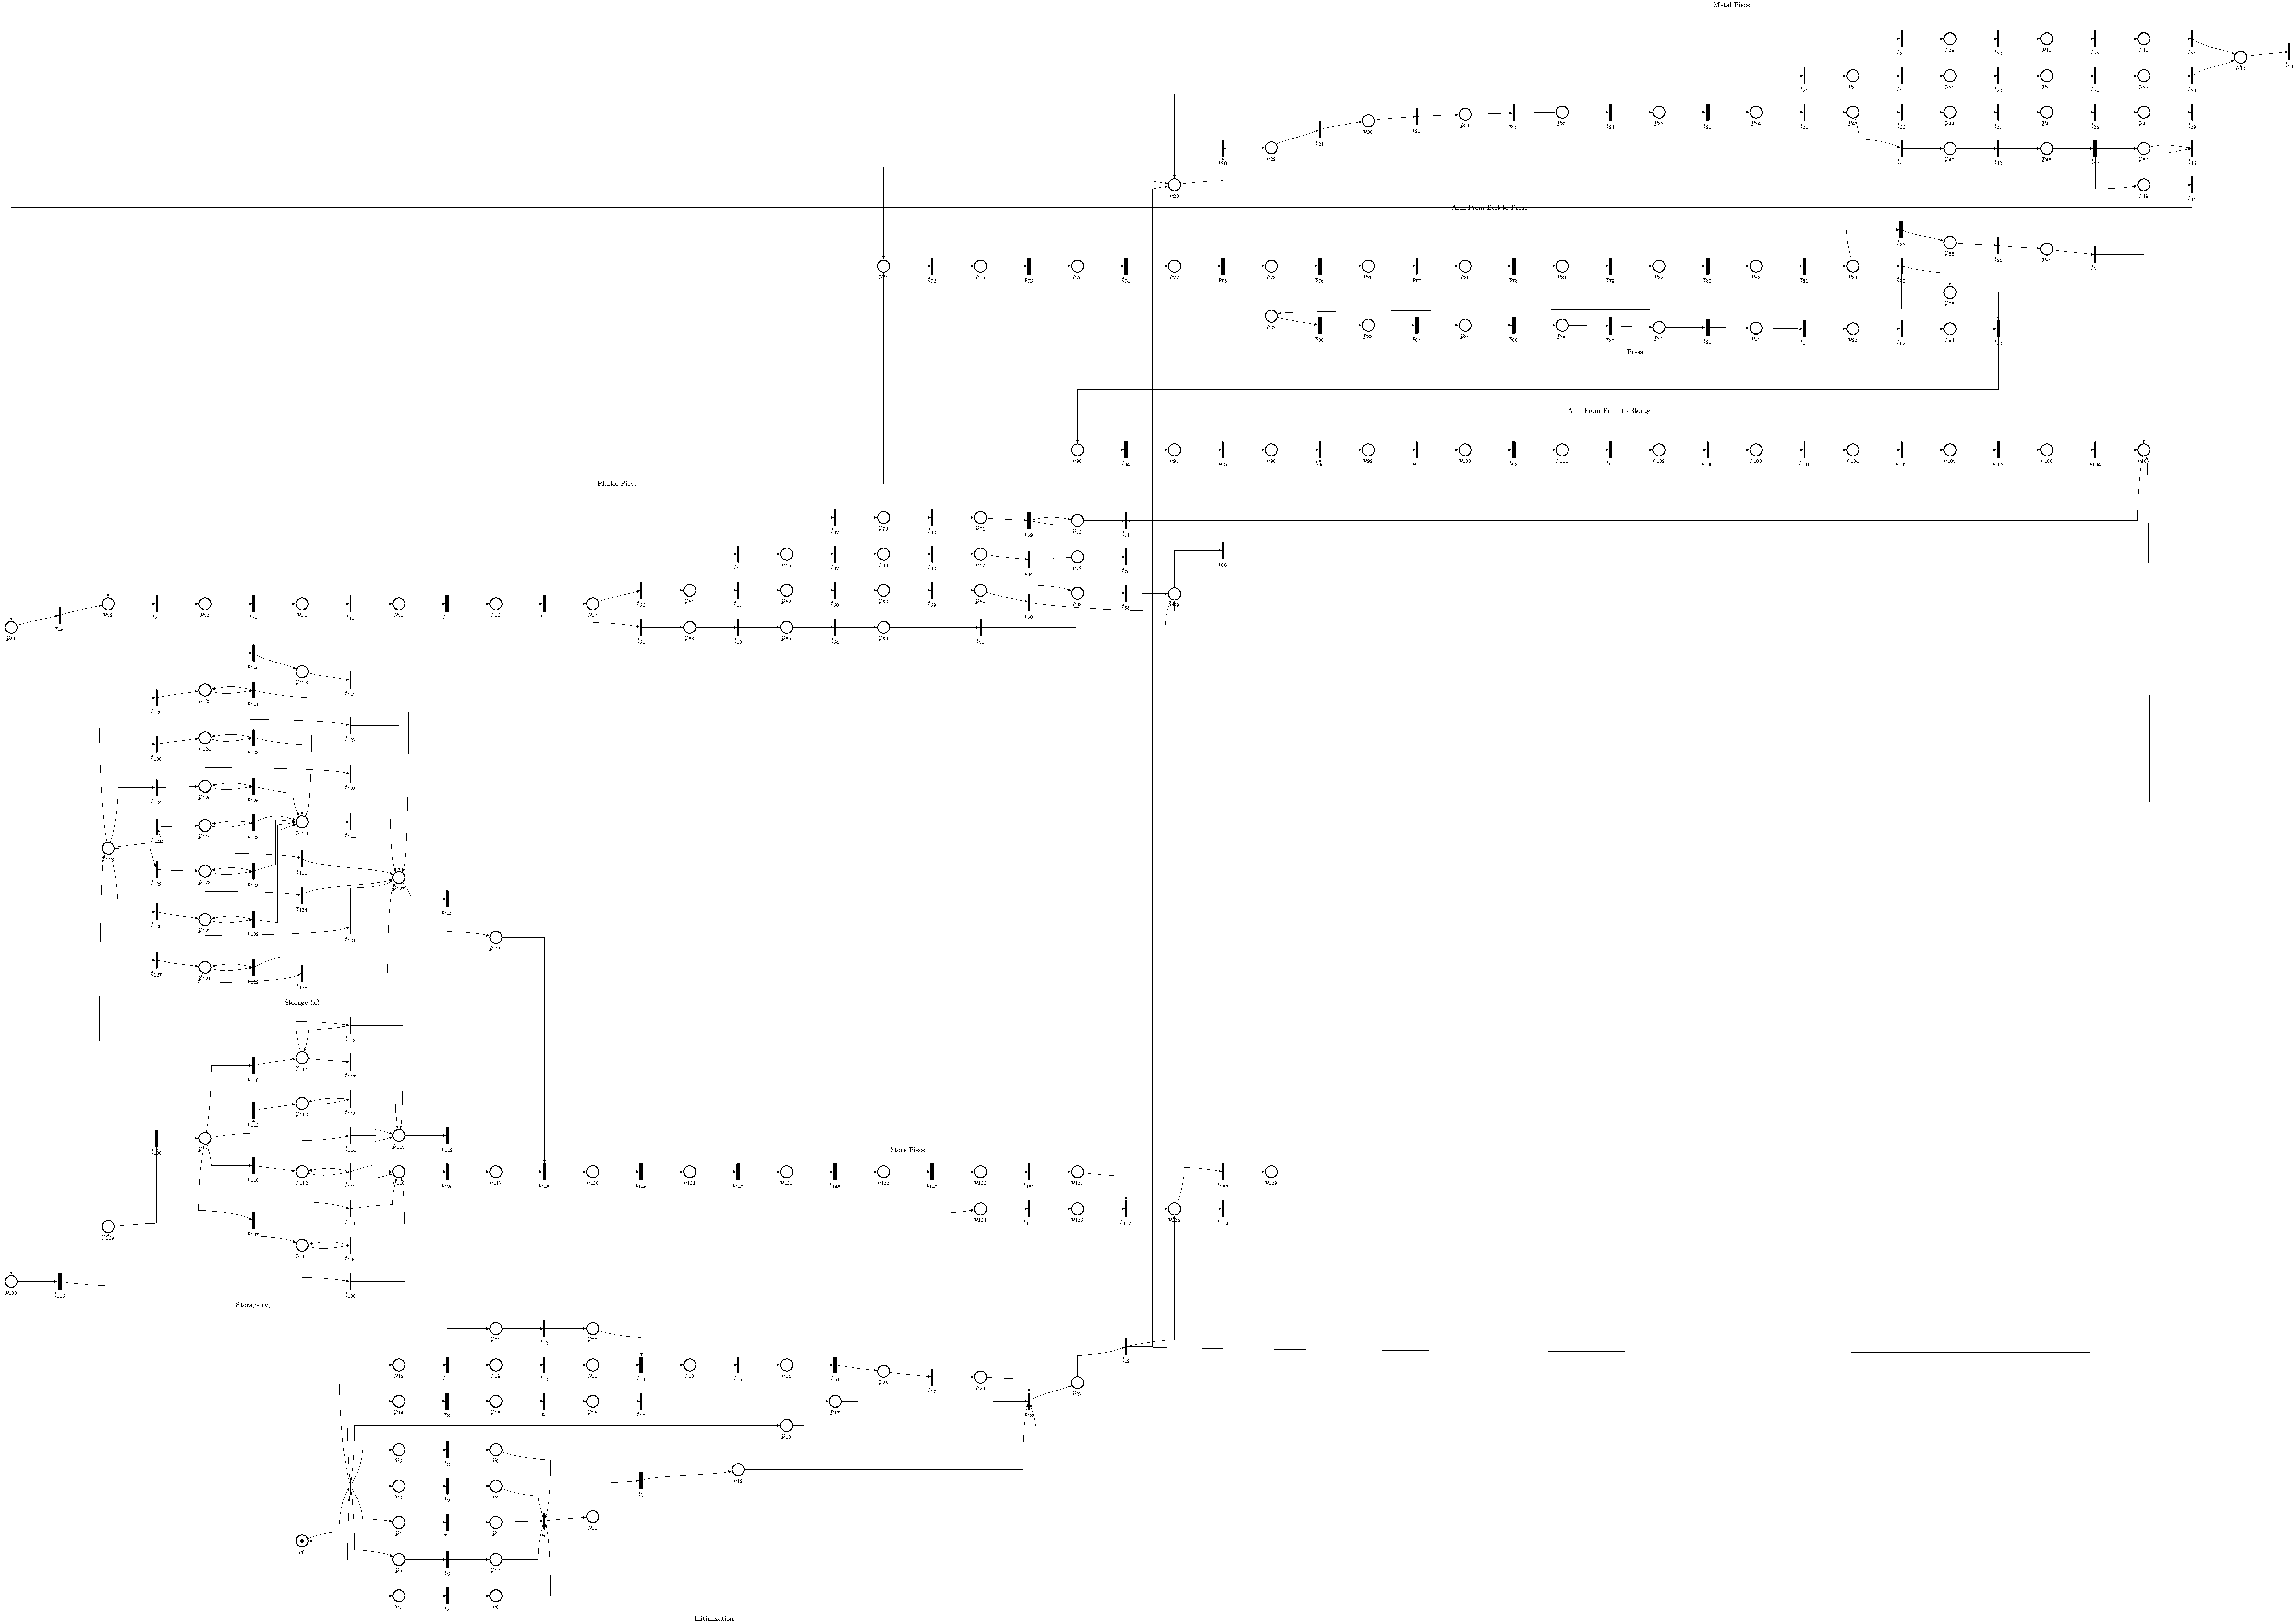
\includegraphics[height=1.28\textheight]{../../figures/petriNet/complete/complete.tikz}}
% \centerline{\resizebox{!}{1.2\textheight}{\begin{tikzpicture}[>=latex',line join=bevel,]
%%
\begin{scope}
  \pgfsetstrokecolor{black}
  \definecolor{strokecol}{rgb}{1.0,1.0,1.0};
  \pgfsetstrokecolor{strokecol}
  \definecolor{fillcol}{rgb}{1.0,1.0,1.0};
  \pgfsetfillcolor{fillcol}
\end{scope}
  \node (x13) at (820.63bp,204.75bp) [draw,circle, double,place, label=above:,rotate=0] {$x_{13}$};
  \node (x12) at (623.63bp,229.75bp) [draw,,circle, label=above:,rotate=0] {$x_{12}$};
  \node (x8) at (623.63bp,531.75bp) [draw,circle, double,place, label=above:,rotate=0] {$x_{8}$};
  \node (x2) at (413.63bp,294.75bp) [draw,,circle, label=above:,rotate=0] {$x_{2}$};
  \coordinate (init) at (28.63bp,208.75bp);
  \node (x9) at (190.63bp,75.748bp) [draw,,circle, label=above:,rotate=0] {$x_{9}$};
  \node (x11) at (518.63bp,229.75bp) [draw,,circle, label=above:,rotate=0] {$x_{11}$};
  \node (x10) at (302.63bp,75.748bp) [draw,circle, double,place, label=above:,rotate=0] {$x_{10}$};
  \node (x3) at (518.63bp,363.75bp) [draw,,circle, label=above:,rotate=0] {$x_{3}$};
  \node (x0) at (93.63bp,208.75bp) [draw,,circle, label=above:,rotate=0] {$x_{0}$};
  \node (x1) at (242.63bp,358.75bp) [draw,,circle, label=above:,rotate=0] {$x_{1}$};
  \node (x6) at (190.63bp,208.75bp) [draw,,circle, label=above:,rotate=0] {$x_{6}$};
  \node (x7) at (302.63bp,234.75bp) [draw,,circle, label=above:,rotate=0] {$x_{7}$};
  \node (x4) at (715.63bp,290.75bp) [draw,,circle, label=above:,rotate=0] {$x_{4}$};
  \node (x5) at (820.63bp,376.75bp) [draw,circle, double,place, label=above:,rotate=0] {$x_{5}$};
  \draw [-Latex] (x4) ..controls (740.45bp,270.42bp) and (776.04bp,241.27bp)  .. (x13);
  \definecolor{strokecol}{rgb}{0.0,0.0,0.0};
  \pgfsetstrokecolor{strokecol}
  \draw (763.63bp,274.25bp) node {\scriptsize $\uparrow$1$\uparrow$2$\downarrow$3 \{3\}};
  \draw [-Latex] (x2) ..controls (440.38bp,278.19bp) and (476.09bp,256.08bp)  .. (x11);
  \draw (464.63bp,284.25bp) node {\scriptsize $\uparrow$1 \{3\}};
  \draw [-Latex] (x0) ..controls (125.39bp,240.72bp) and (195.71bp,311.52bp)  .. (x1);
  \draw (142.63bp,286.25bp) node {\scriptsize $\uparrow$2 \{0\}};
  \draw [-Latex] (x11) ..controls (549.13bp,229.75bp) and (579.37bp,229.75bp)  .. (x12);
  \draw (569.63bp,239.25bp) node {\scriptsize $\downarrow$1$\downarrow$2$\downarrow$3 \{3\}};
  \draw [-Latex] (x6) ..controls (219.89bp,215.54bp) and (258.12bp,224.42bp)  .. (x7);
  \draw (242.63bp,234.25bp) node {\scriptsize $\uparrow$1$\uparrow$2 \{1, 3\}};
  \draw [-Latex] (x1) ..controls (280.92bp,344.42bp) and (357.34bp,315.82bp)  .. (x2);
  \draw (302.63bp,351.25bp) node {\scriptsize $\downarrow$1$\uparrow$3 \{0\}};
  \draw [-Latex] (x0) ..controls (120.39bp,208.75bp) and (149.16bp,208.75bp)  .. (x6);
  \draw (142.63bp,218.25bp) node {\scriptsize $\downarrow$1 \{1, 3\}};
  \draw [-Latex] (init) ..controls (58.462bp,208.75bp) and (65.783bp,208.75bp)  .. (x0);
  \draw [-Latex] (x2) ..controls (440.34bp,312.3bp) and (478.01bp,337.06bp)  .. (x3);
  \draw (464.63bp,350.25bp) node {\scriptsize $\downarrow$2$\downarrow$3 \{0, 1\}};
  \draw [-Latex] (x3) ..controls (540.89bp,399.37bp) and (586.69bp,472.65bp)  .. (x8);
  \draw (569.63bp,481.25bp) node {\scriptsize $\uparrow$1 \{1\}};
  \draw [-Latex] (x12) ..controls (650.18bp,247.35bp) and (679.13bp,266.55bp)  .. (x4);
  \draw (672.63bp,280.25bp) node {\scriptsize $\uparrow$3 \{3\}};
  \draw [-Latex] (x4) ..controls (740.8bp,311.36bp) and (777.58bp,341.49bp)  .. (x5);
  \draw (763.63bp,353.25bp) node {\scriptsize $\uparrow$1$\downarrow$3 \{0\}};
  \draw [-Latex] (x9) ..controls (218.67bp,75.748bp) and (251.27bp,75.748bp)  .. (x10);
  \draw (242.63bp,85.248bp) node {\scriptsize $\uparrow$1$\downarrow$2$\downarrow$3 \{2\}};
  \draw [-Latex] (x7) ..controls (330.95bp,250.05bp) and (371.05bp,271.73bp)  .. (x2);
  \draw (361.63bp,286.25bp) node {\scriptsize $\downarrow$1$\uparrow$3 \{1, 3\}};
  \draw [-Latex] (x3) ..controls (560.69bp,348.16bp) and (653.99bp,313.59bp)  .. (x4);
  \draw (623.63bp,338.25bp) node {\scriptsize $\uparrow$3 \{0\}};
  \draw [-Latex] (x0) ..controls (116.29bp,177.68bp) and (157.03bp,121.81bp)  .. (x9);
  \draw (142.63bp,175.25bp) node {\scriptsize $\downarrow$1$\uparrow$2$\uparrow$3 \{2\}};
%
\end{tikzpicture}
}}
\end{figure}

\KOMAoptions{paper=a4,paper=portrait}
\recalctypearea

%%% Local Variables:
%%% mode: latex
%%% TeX-master: "../monografia"
%%% End:
